\documentclass[10pt,a4paper]{article}
\usepackage[utf8]{inputenc}
\usepackage{amsmath}
\usepackage{amsfonts}
\usepackage{amssymb}
\usepackage{graphicx}
\usepackage[swedish]{babel}
\usepackage[utf8]{inputenc}

\graphicspath{}

\author{
  \texttt{Sebastian Bångerius}
  \and
  \texttt{Andreas Nordberg}
  \and
  \texttt{Villiam Rydfalk}
  \and
  \texttt{Anton Silfver}
}

\begin{document}
\pagenumbering{gobble}

\title{Studsmatta}
\maketitle

\cleardoublepage

\tableofcontents

\clearpage

\section{Syfte}
\pagenumbering{arabic}
\setcounter{page}{3}

Syftet med vår rapport är att genom att betrakta en studsmatta som ett idealiserat svängningssystem betrakta dess egenskaper och dra relevanta slutsatser angående dess beteende och egenskaper och vilka faktorer som påverkar dessa.

\subsection{Mål}

Målet med vår rapport är att genom vår ökade förståelse om hur man kan påverka insignalen till vårt system för att få utsignalen att bete sig på önskat sätt. Till exempel hur man bör gå till väga för att få största möjliga utsignal, med andra ord hoppa så högt som möjligt på en studsmatta.

\section{Bakgrund}

Vi har i denna rapport valt att modellera en person som hoppar på en studsmatta som en linjärt system för att undersöka dess egenskaper. Vi ville välja ett linjärt för att analysera deras egenskaper men samtidigt använda oss av en mycket värklighetstrogen modell som inte kräver så mycket idealisering för att kunna representeras som just en linjärt svängningssystem.

\subsection{Vad är ett linjärt system?}

Många är inte förvånade att höra att definitionen av ett linjärt system är att systemet ska vara för det första homogent och för det andra additivt. Men hur defineras det inom kontexten av system, vad innebär det och vilka egenskaper medförs av att ett system är linjärt? Det är så att om

\begin{equation}
x(t) = a*x_1(t) + b*x_2(t)\rightarrow y(t) = a*y_1(t) + b*y_2(t)
\end{equation}
stämmer så är systemet linjärt

\newpage
\section{Vårt LTI system}

\begin{figure}[ht]
\caption{En enkel bild av vårt system}
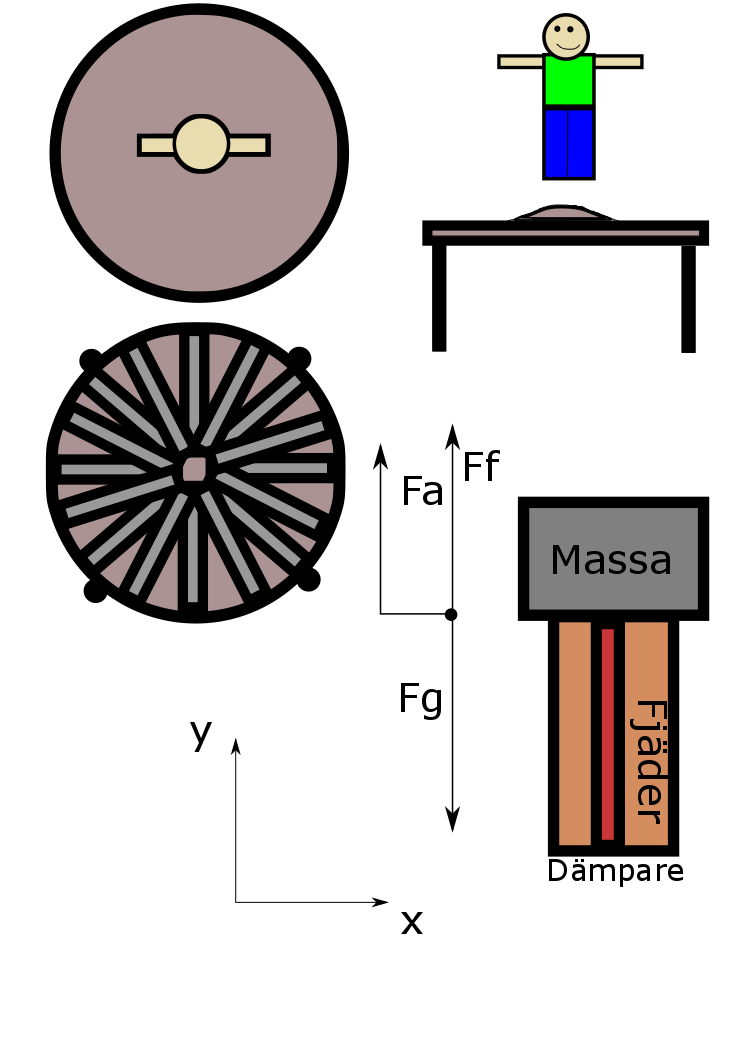
\includegraphics[scale=0.4]{Bild}
\end{figure}
\clearpage

Den enkla bilden ger en överblick av vårt system. Studsmattan är helt cirkulär och har fjädrar som sitter radiellt från kanten in i mitten symmetriskt runt om.

\subsection{Fysik 1}

\subsection{Fysik 2}

\subsection{Fysik 3}

\subsection{Slutgiltig diff.ekv}

\end{document}